\RequirePackage{plautopatch}  % pLaTeX または upLaTeX のとき
%\documentclass[uplatex,dvipdfmx,titlepage,a4j]{jsarticle}% upLaTeX のとき
\documentclass[dvipdfmx,titlepage,a4j]{jsarticle}  % pLaTeX のとき
\usepackage{listings,jvlisting}
\usepackage{amsmath,amssymb}
\usepackage{graphicx}
\usepackage[yen]{okuverb}
\usepackage{r04ec-exp}
\usepackage{here}
\usepackage{ascmac}
\usepackage{fancybox}
\usepackage{fancyvrb}
\usepackage{fancyhdr}
\usepackage{lastpage}
\usepackage{cases}

\fancypagestyle{foot}
{
\fancyhead[L]{}
\fancyhead[C]{数値シミュレーション}
\fancyhead[R]{}
% \fancyfoot[C]{\thepage / \pageref{LastPage}}
\renewcommand\headrulewidth{0.4pt}
}

%ここからソースコードの表示に関する設定
\lstset{
  language={C++},
  basicstyle={\ttfamily},
  identifierstyle={\small},
  commentstyle={\smallitshape},
  keywordstyle={\small\bfseries},
  ndkeywordstyle={\small},
  stringstyle={\small\ttfamily},
  frame={tb},
  tabsize={2},
  breaklines=true,
  columns=[l]{fullflexible},
  numbers=left,
  xrightmargin=0zw,
  xleftmargin=3zw,
  numberstyle={\scriptsize},
  stepnumber=1,
  numbersep=1zw,
  lineskip=-0.5ex
}

\renewcommand{\lstlistingname}{リスト}
%ここまでソースコードの表示に関する設定

\title{数値シュミレーション}
% 学年・番号
\grade{4年42番}%
% 氏名
\author{鷲尾 優作}
% 班(後期は班に分かれて実験をする.そのときは,ここに班番号を記入する.)
\team{}
% 提出日
\date{2022年10月3日}
% 実験日
\expdate{2022年10月20日}
% 共同実験者
% グループに分かれて実験をするテーマでは,グループメンバーの番号名前を書く.
\coauthor{}
%
%記載例:
%\coauthor{%
%  2番 & 新潟 花子\\
%  11番 & 三条 次郎}
%%

\begin{document}
\pagestyle{foot}

\maketitle

\section{目的}
これまでの実験・講義では解析的に系の挙動を明らかにすることができるモデルを扱ってきた.

しかしながら,二重振り子をはじめとした複雑な系では従来の解析方法が適用できない場合が存在し,
この場合,エネルギ式を用いての運動方程式の導出や数値モデルを利用した運動シミュレーションが有効とされている.
同技術には,系の挙動の解析のみならず,安定化や安全性の向上に用いる制御器の制御パラメータの導出がコンピュータ上で行える利点がある.

ここでは,電気系・力学系のシミュレーションモデルをScilab上で構成し,解析結果の有効性確認方法・対象の制御パラメータの調整法を確認する.

\section{バネ-マス-ダンパ系のシミュレーション}
本来数値シミュレーションを必要とするのはより複雑な系の解析であるが,ここでは単純なバネ-マス-ダンパ系のシミュレーションモデルを
構成し,モデルの構成方法・出力の評価が正しく実施できることを確認する.

天井の固定点からバネ$k$[kg/s$^2$]でダンパ$c$[kg/s]で支持された質量$m$[kg]から
なる系を考える.質量の運動は上下方向のみとし,重力と空気抵抗の影響は受けないものとする.
この系に対し,ステップ状の外力$f(t) = f_o \cdot u(t)$ [kg $\cdot$ cm / s$^2$]
が質量に加わった場合について調べる.

\subsection{バネ-マス-ダンパ系の運動方程式の導出}
質量$m$の変位$x(t)$とすると,この物体の加速度は$\frac{d^2x(t)}{dt^2}$であるから,
運動の法則及び力の釣合より,運動方程式は(\ref{eq:bane-undou})式のように決定される.
\begin{eqnarray}
  m \frac{d^2x(t)}{dt^2} &=& f(t) - kx - c \frac{dx(t)}{dt} \nonumber \\
  &=& f_o \cdot u(t) - kx - c \frac{dx}{dt} \label{eq:bane-undou}
\end{eqnarray}

\subsection{構成したシミュレーションモデル}

(\ref{eq:bane-undou})式を解析し,変位$x(t)$[cm]及び速度$v(t)$[cm/s]を出力するシミュレーションモデルを構成する.

(\ref{eq:bane-undou})式の左辺が$x(t)$の2階微分項のみとなるよう変形した,(\ref{eq:bane-henkei})式を考える.
\begin{eqnarray}
  \frac{d^2x(t)}{dt^2} &=&  \frac{1}{m} f_o \cdot u(t) - \frac{k}{m} x - \frac{c}{m} \frac{dx(t)}{dt} \label{eq:bane-henkei}
\end{eqnarray}

$v(t) = \int \frac{d^2x(t)}{dt^2}$,$x(t) = \int v(t)$であるから,
(\ref{eq:bane-henkei})式を積分して速度$v(t)$[cm/s]が,更に再度積分して変位$x(t)$[cm]が求まる.
また,右辺に存在する定数$\frac{1}{m}$,$- \frac{k}{m}$,$- \frac{c}{m}$は$x(t)$に対して積の構造となっているため,線形なゲイン倍として表現できる.

これらの情報から,Scilabに用意されている積分器$\frac{1}{s}$及びゲイン倍ブロック用いれば,
ステップ入力に対してのモデルを構成できることがわかる.
作成したモデルを図\ref{fig:bane-model.png}に示す.

\begin{figure}[H]
  \centering
  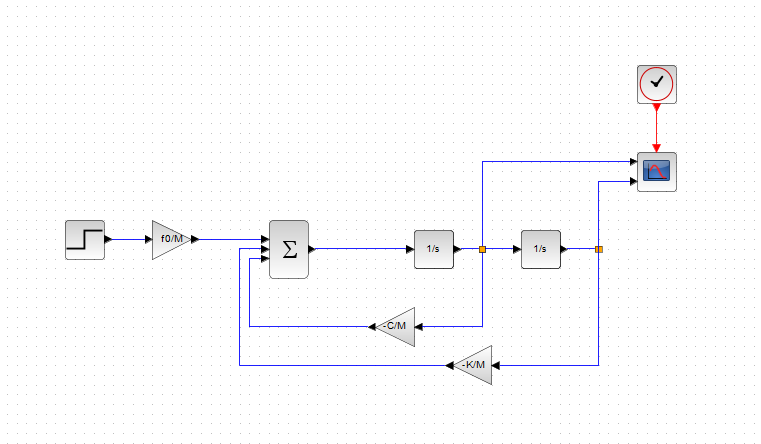
\includegraphics[width=10cm]{../graph/bane-model.png}
  \caption{作成したシミュレーションモデル}
  \label{fig:bane-model.png}
\end{figure}

このとき,左側の積分器の出力が$v(t)$であり,右側の積分器の出力が$x(t)$である.

\subsection{シミュレーションパラメータ値の計算}
使用した各定数は参考文献[1]の指示に従い決定した.
実際に使用した値はそれぞれ次のとおりである.
\begin{itemize}
  \item $m = 出席番号 \times 100$ = 420[kg]
  \item $k = \frac{|150 + (出席番号 - 25)^2 \times 50|}{10} = 1460$[kg/s$^2$]
  \item $c = 650 - (出席番号 - 25)^2 = 361$[kg/s]
  \item $f_o = 300$[kg $\cdot$ cm / s$^2$]
\end{itemize}

\subsection{シミュレーション結果}
各定数を設定したモデルに対し,シミュレーション時間0[s]においてステップ入力1を与え,出力を得た.
変位$x(t)$[cm]及び速度$v(t)$[cm/s]の時間に対するグラフを図\ref{fig:bane-graph.png}に示す.

\begin{figure}[H]
  \centering
  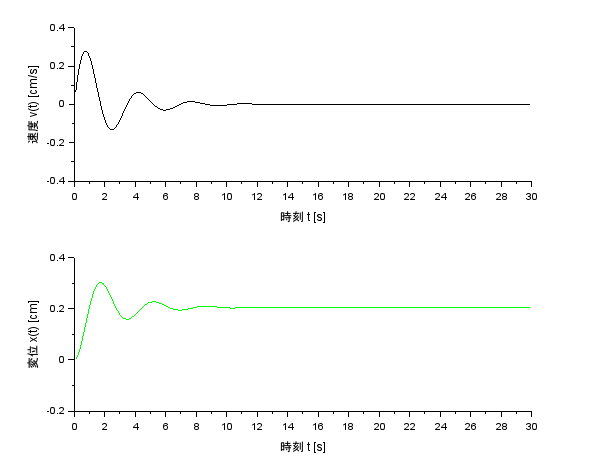
\includegraphics[width=10cm]{../graph/bane-graph.png}
  \caption{系の時間応答シミュレーション結果}
  \label{fig:bane-graph.png}
\end{figure}

\subsection{シミュレーション結果の解析}
まず,質量は正のステップ入力に対し,$x(t)$が正の方向に変位し,また,加速により$v(t)$が正となることは間違いない.
少なくともこの観点には,図2の出力は沿った結果となっている.

次に,定常応答について評価する.
定常応答は,$t \rightarrow \infty$となったときの$x(t)$及び$v(t)$である.
質量は最終的に静止するはずであるから,$v(t)$の定常応答は0となるはずである.
一方,$x(t)$の定常応答は,バネによる弾性力とダンパによる抵抗力のバランスによって決定される.
$x(t)$の定常応答$x_\infty$は,$x_\infty = \frac{f_o}{k}$とすると,
$v(t)$が0となればダンパの抵抗力は発生しなくなることを考えれば,$x_\infty = \frac{300}{1460} = 0.205$[cm]となる.
これら2つの定常応答に対して,図2の出力は沿った結果となっている.

最終的にシミュレーションモデルの結果が正しいか判断するには,これに加え収束までの時間と,周波数について検討する必要があると考えられる.
しかし,今回は時間が足りなかったため,これらの検討は行わなかった.
したがってダンパ成分に対する評価が不十分である.

\section{天井クレーンの制御シミュレーション}
数値シミュレーションによる系の制御の実践として,複数の要素が含まれ解析が難しい天井クレーンの安定化を考える.

図 に天井クレーンの構造を示す.
高さ方向$y$,横方向$x$,奥行方向$z$の3軸を考えたとき,一般的な天井クレーンは吊り荷の
移動機構としてそれぞれ巻き上げ機構,トロリ,クレーンガーターを備える.

今回のシミュレーションモデルでは,簡略化のため,クレーンガーター,巻き上げ機構は固定とし,トロリの移動のみを考慮する.
吊り下げる荷重,ロープ長は任意の長さで固定されているものし,
座標系はトロリの移動方向$x$軸,鉛直下向きを$y$軸とする.

このとき,トロリの質量$M$[kg],吊り荷の質量$m$[kg],ロープの長さ$l$[m],
ロープ根本の粘性係数は$\mu$[kg$\cdot m^2$/s]であるとすると,シミュレーションに用いる天井クレーンは
図 のようにモデル化できる.

また,ロープは無視できる質量であるとし,
トロリの変位$x(t)$は右方向を正,吊り荷の揺れ角$\theta(t)$は反時計回りを正とする.
トロリと吊り荷はそれぞれ相互に影響しあい,吊り荷の揺れ角$\theta(t)$はトロリの変位$x(t)$に依存し発生・抑制されるものと考える.

\subsection{天井クレーンの吊り荷部分の運動方程式の導出}
天井クレーンの吊り荷の制振が目的であるから,この部分の運動方程式を導出する.
吊り荷の一般化座標$q(t) = \theta(t)$として,ラグランジュ法を用いて運動方程式を導出する.

運動エネルギ,位置エネルギ,散逸エネルギ,外力によるエネルギの総和を考える.
それぞれ$T$,$U$,$F$,$\tau_i$とし,
ラグラジアン$L = T - U$から,ラグランジュの運動方程式を次のように定義する.
\begin{equation}
  \frac{d}{dt} \frac{\partial T}{\partial \dot{q}} - \frac{\partial T}{\partial q} + \frac{\partial F}{\partial \dot q} + \frac{\partial U}{\partial \dot q} = \tau \nonumber
\end{equation}

外力$\tau$=0として,吊り荷のラグランジュの運動方程式は式(\ref{eq:lagrange})と表せる.
\begin{equation}
  \frac{d}{dt} \frac{\partial T}{\partial \dot{q}} - \frac{\partial T}{\partial q} + \frac{\partial F}{\partial \dot q} + \frac{\partial U}{\partial \dot q} = 0 \label{eq:lagrange}
\end{equation}

各エネルギを導出するため,吊り荷の中心座標を導出する.
ロープが曲がることはないと仮定すると,吊り荷の中心座標$(G_x, G_y)$は,トロリの中心座標$x$と吊り荷の角度$\theta$,ロープ長$l$によって決定される.
このとき,$(G_x, G_y)$は次のとおりである.

\begin{equation}
  \begin{cases}
    G_x = l sin(\theta(t)) + x \nonumber \\
    G_y = l cos(\theta(t))
  \end{cases}
\end{equation}

また,この微分は次のとおりである.
\begin{equation}
  \begin{cases}
    \dot{G_x} = l \dot{\theta(t)} cos(\theta(t)) + \dot x \nonumber \\
    \dot{G_y} = -l \dot{\theta(t)} sin(\theta(t))
  \end{cases}
\end{equation}

中心座標を考慮して吊り荷の運動エネルギ$T$を導出する.
\begin{eqnarray}
  T &=& \frac{1}{2} m (\dot{G_x}^2 + \dot{G_y}^2) + \frac{1}{2}M\dot{x}^2\nonumber \\
  &=& \frac{1}{2} m [ \{l \dot{\theta(t)} cos(\theta(t)) + \dot x\}^2 + \{ -l \dot{\theta(t)} sin(\theta(t))\}^2 ] + \frac{1}{2}M\dot{x}^2 \nonumber \\
  &=& \frac{1}{2} m [\{ \dot x^2 + 2 l \dot{x} \dot{\theta(t)} cos(\theta(t)) + l^2 \dot{\theta(t)}^2 cos^2(\theta(t)) \} + l^2 \dot{\theta(t)}^2 sin^2(\theta(t))] + \frac{1}{2}M\dot{x}^2 \nonumber \\
  &=& \frac{1}{2} m [\dot x^2 + 2 l \dot{x} \dot{\theta(t)} cos(\theta(t)) + l^2 \dot{\theta(t)}^2 \{ cos^2(\theta(t)) + sin^2(\theta(t)) \}] + \frac{1}{2}M\dot{x}^2 \nonumber \\
  &=& \frac{1}{2} m [\dot x^2 + 2 l \dot{x} \dot{\theta(t)} cos(\theta(t)) + l^2 \dot{\theta(t)}^2] + \frac{1}{2}M\dot{x}^2 \nonumber \\
  &=& \frac{1}{2} m \dot x^2 + m l \dot{x} \dot{\theta(t)} cos(\theta(t)) + \frac{1}{2} m l^2 \dot{\theta(t)}^2 + \frac{1}{2}M\dot{x}^2 \nonumber \\
  &=& \frac{1}{2} (M + m)\dot x^2 + m l \dot{x} \dot{\theta(t)} cos(\theta(t)) + \frac{1}{2} m l^2 \dot{\theta(t)}^2 \label{eq:energy}
\end{eqnarray}

同様に,位置エネルギ$U$,散逸エネルギ$F$は次のとおりである.
\begin{eqnarray}
  U &=& mg(l - G_y) \nonumber \\
  &=& mg(l - l cos(\theta(t))) \nonumber \\
  &=& mgl(1 - cos(\theta(t)) \label{eq:potential}\\
\end{eqnarray}

\begin{eqnarray}
  F &=& \frac{1}{2} \mu  \dot{\theta(t)}^2 \label{eq:friction}
\end{eqnarray}

式(\ref{eq:energy}),(\ref{eq:potential}),(\ref{eq:friction})をラグランジュの運動方程式(\ref{eq:lagrange})に代入し,エネルギ式を導く.

ここで各項は,
\begin{eqnarray}
  \frac{d}{dt} \frac{\partial T}{\partial \dot{q}} &=& m l^2 \theta(t) + m l \dot(x) cos(\theta(t)) \nonumber \\
  \frac{\partial T}{\partial \dot{q}} &=&  -m l \dot x \dot{\theta(t)}^2 sin(\theta(t))\nonumber \\
\end{eqnarray}

\begin{eqnarray}
  \frac{d}{dt} \frac{\partial F}{\partial \dot{q}} &=&  \mu \dot{\theta(t)} \nonumber \\
  \frac{\partial U}{\partial \dot{q}} &=&  mgl sin(\theta(t)) \nonumber \\
\end{eqnarray}

であるから,求める運動方程式は
\begin{eqnarray}
  \frac{d}{dt} \frac{\partial T}{\partial \dot{q}} - \frac{\partial T}{\partial q} + \frac{\partial F}{\partial \dot q} + \frac{\partial U}{\partial \dot q} = 0 \nonumber \\
  m l^2 \theta(t) + m l \dot x cos(\theta(t)) + m l \dot x \dot{\theta(t)}^2 sin(\theta(t)) + \mu \dot{\theta(t)} + mgl sin(\theta(t)) = 0 \nonumber \\
\end{eqnarray}

\subsection{シミュレーションパラメータの計算}
天井クレーンの各シミュレーションパラメータは参考文献[1]の指示に従い決定した.
実際にシミュレーションに使用した値はそれぞれ次のとおりである.
\begin{itemize}
  \item $m = 0.5 + (\frac{出席番号 - 25}{10})^2 = 3.39$
  \item $l = 0.16 + (出席番号 \times 0.04) = 1.84$
  \item $\alpha_1 = 37.2$
  \item $\alpha_2 = 1980$
  \item $\beta = 180$
  \item $\mu = 1.22 \times  10^{-3}$
\end{itemize}

\subsection{設計仕様を満たすPID制御器の設計とシミュレーション結果}
設計したPID制御器について述べる.
今回のシミュレーションでは,目標位置に向けてトロリの制動速度を制御するPID制御器,吊り荷の揺れ角によってトロリの速度を制御するPID制御器の2つを考える.

前者は,目標位置が近づくにつれてトロリの制動速度を減速させることで,目標位置に到達するまでの時間を効率的に短縮する等の役割を担う.
後者は,吊り荷の揺れ角が大きくなるにつれてトロリの速度を減速させることで,吊り荷の揺れ角を小さくする等の役割を担う.


\section{感想}

\begin{thebibliography}{99}
  \bibitem{ataka} 佐藤 拓史、実験テキスト「数値シュミレーション」、(2022年),
\end{thebibliography}

\end{document}